\documentclass{article}
\linespread{1.3}
\usepackage[margin=50pt]{geometry}
\usepackage{amsmath, amsthm, amssymb, amsthm, tikz, fancyhdr, float, graphicx, spverbatim, systeme}
\pagestyle{fancy}
\renewcommand{\headrulewidth}{0pt}
\newcommand{\changefont}{\fontsize{15}{15}\selectfont}

\fancypagestyle{firstpageheader}{
  \fancyhead[R]{
    \changefont
    \parbox[t]{4cm}{ % Adjust width as needed
      Michael Huang\\
      EN.555.644.81\\
      Final
    }
  }
}

\begin{document}

\thispagestyle{firstpageheader}
{\Large 

\section*{13.}

\subsection*{(a)} 

The initial correct response to Question 8 was C: \(c = S_0 N(d_1) - Ke^{-rt} N(d_2)\). Using this terminology, we can flip accordingly, i.e. that
\[
  \boxed{\mathbf{p = Ke^{-rT} N(-d_2) - S_0 N(-d_1)}}
\]

\subsection*{(b)}

The formulas for \(d_1\) and \(d_2\) are as following:
\[
  \boxed{\mathbf{d_1 = \frac{\ln(\frac{S_0}{K}) + (r + \frac{\sigma^2}{2})T}{\sigma \sqrt{T}}}}
\]
and 
\[
  \boxed{\mathbf{d_2 = \frac{\ln(\frac{S_0}{K}) + (r - \frac{\sigma^2}{2})T}{\sigma \sqrt{T}}}}
\]
Naturally, \(S_0\) is the initial stock price, \(K\) is the strike price of the option, \(r\) is the risk-free rate, \(\sigma\) is the volatility, and \(T\) is the time to expiry. Finally, regarding the relationship of the parameters to each other, we know that \(\boxed{\mathbf{d_2 = d_1 - \sigma \sqrt{T}}}\).

\subsection*{(c)}
The simple enhancement here is to replace the straight-up initial stock price with its present value discounted by the dividends, so we use the dividend yield \(q\) and replace all \(S_0\) with \(S_0 e^{-qT}\). Starting with the call option formula:
\[
  \boxed{\mathbf{c = S_0e^{-qT} N(d_1) - Ke^{-rT} N(d_2) }}
\]
And accordingly for \(d_1\) and \(d_2\): 
\[
  d_1 = \frac{\ln(\frac{S_0e^{-qT}}{K}) + (r + \frac{\sigma^2}{2})T}{\sigma \sqrt{T}}
\]
\[
  = \frac{\ln(\frac{S_0}{K}) - qT + (r + \frac{\sigma^2}{2})T}{\sigma \sqrt{T}}
\]
\[
  \boxed{\mathbf{d_1 = \frac{\ln(\frac{S_0}{K}) + (r - q + \frac{\sigma^2}{2})T}{\sigma \sqrt{T}}}}
\]
and accordingly, 
\[
  \boxed{\mathbf{d_2 = \frac{\ln(\frac{S_0}{K}) + (r - q - \frac{\sigma^2}{2})T}{\sigma \sqrt{T}}}}
\]

}
{\Large 

\section*{14.}

\subsection*{(a)}

With \(dS = \mu S dt + \sigma S dz\), and first applying Ito's lemma, we have 
\[
  df = (\frac{\partial f}{\partial S} \mu S + \frac{\partial f}{\partial t} + \frac{1}{2} \frac{\partial^2 f}{\partial S^2}\sigma^2 S^2) dt + \frac{\partial f}{\partial S} \sigma S dz
\]
So using the model of constructing the riskless portfolio, we short one unit of the derivative and long \(\frac{\partial f}{\partial S}\) of the underlying, and take the change in porfolio value:
\[
  \Pi = -f + \frac{\partial f}{\partial S} S
\]
\[
  \Delta \Pi = - \Delta f + \frac{\partial f}{\partial S} \Delta S
\]
\[
  = - df + \frac{\partial f}{\partial S} dS
\]
Substitute accordingly:
\[
  \Delta \Pi = - (\frac{\partial f}{\partial S} \mu S + \frac{\partial f}{\partial t} + \frac{1}{2} \frac{\partial^2 f}{\partial S^2}\sigma^2 S^2) dt - \frac{\partial f}{\partial S} \sigma S dz + \frac{\partial f}{\partial S} (\mu S dt + \sigma S dz)
\]
\[
  \Delta \Pi = - (\frac{\partial f}{\partial t} + \frac{1}{2} \frac{\partial^2 f}{\partial S^2}\sigma^2 S^2) dt
\]
Here, we apply the argument that a riskless portfolio must earn the risk-free rate, otherwise we would be able to arbitrage in this riskless portfolio, i.e. 
\[
  \Delta \Pi = r \Pi dt
\]
\[
  - (\frac{\partial f}{\partial t} + \frac{1}{2} \frac{\partial^2 f}{\partial S^2}\sigma^2 S^2) dt = r (-f + \frac{\partial f}{\partial S} S) dt
\]
\[
  - (\frac{\partial f}{\partial t} + \frac{1}{2} \frac{\partial^2 f}{\partial S^2}\sigma^2 S^2) = r (-f + \frac{\partial f}{\partial S} S)
\]
\[
  - \frac{\partial f}{\partial t} - \frac{1}{2} \frac{\partial^2 f}{\partial S^2}\sigma^2 S^2 = -rf + r\frac{\partial f}{\partial S} S
\]
\[
  \boxed{ \mathbf{\frac{\partial f}{\partial t} + rS \frac{\partial f}{\partial S} + \frac{1}{2} \sigma^2 S^2 \frac{\partial^2 f}{\partial S^2} = rf}}
\]
exactly as we sought to find.

\subsection*{(b)}

When \(t = T\), i.e. the option is at expiry, the value of a European put has the following boundary condition:
\[
  \boxed{\mathbf{f = \max(K - S, 0)}}
\]

}
{\Large 

\section*{15.}

\subsection*{(a)}

The Principle of Risk Neutral Valuation is that as stated in the problem statement, the Black-Scholes-Merton differential equation relies only on time, the stock price, volatility and the risk-free rate. In application, this means that we can price real-world derivatives under the simplified model of the risk-neutral world (where both the expected return of all underlyings and the dicsount rate for all cash flows are equivalent to the risk free rate) and these can be considered equivalent. To get to this risk-neutral valuation, we simply set the expected return of the underlying to equal the risk free rate (set \(\mu = r\)), proceed to calculate the payoff accordingly, and then finally discount the payoff back to present time \(t\) using the risk-free rate \(r\). 

\subsection*{(b)}
We use the process as stated above. With the long forward contract on a non-dividend paying stock, we know that the expected payoff is \(S_T - K\). Applying the expected growth to the stock, we have that \(\hat{E}(S_T) = S_0 e^{rT} \), so accordingly for \(T - t\), we get that the expected risk-neutral payoff should actually be \(S e^{r (T - t)} - K\). Finally, we discount this expected payoff to present value to get
\[
  f = e^{-r(T - t)} (S e^{r(T - t)} - K) = \boxed{\mathbf{S - K e^{r(T - t)}}}
\]

\subsection*{(c)}
We have the BSM PDE as 
\[
  \frac{\partial f}{\partial t} + r S \frac{\partial f}{\partial S} + \frac{1}{2} \sigma^2 S^2 \frac{\partial^2 f}{\partial S^2} = rf
\]
With \(f = S - K e^{r(T - t)}\), we calculate the partial derivatives accordingly: \\
- \(\frac{\partial f}{\partial t} = \frac{\partial}{\partial t} f = 0 - Ke^{-r(T-t)} \cdot -r = -r K e^{-r(T - t)} \)  \\
- \(\frac{\partial f}{\partial S} = \frac{\partial}{\partial S} f = 1 - 0 = 1\) \\
- \(\frac{\partial^2 f}{\partial S^2} = \frac{\partial}{\partial S} \frac{\partial f}{\partial S} = 0 \) \\
Now plugging in: 
\[
  \frac{\partial f}{\partial t} + r S \frac{\partial f}{\partial S} + \frac{1}{2} \sigma^2 S^2 \frac{\partial^2 f}{\partial S^2} = rf
\]
\[
  -r K e^{-r(T - t)} + r S \cdot 1 + \frac{1}{2} \sigma^2 S^2 \cdot 0 = rf
\]
\[
  -r K e^{-r(T - t)} + r S + 0 = rf
\]
\[
  r(S - K e^{-r(T - t)}) = rf
\]
which, looking back to part (b), matches exactly as we expected. 

}
{\Large 

\section*{16.}

\subsection*{(a)}

We can treat the futures price like a stock with dividend and set \(q = r = 0.06\) here. The corresponding Black-Scholes equation is therefore derivable as follows:
\[
  \frac{\partial f}{\partial t} + (r - q) S \frac{\partial f}{\partial S} + \frac{1}{2} \sigma^2 S^2 \frac{\partial^2 f}{\partial S^2} = rf
\]
\[
  \frac{\partial f}{\partial t} + (r - q) F \frac{\partial f}{\partial F} + \frac{1}{2} \sigma^2 F^2 \frac{\partial^2 f}{\partial F^2} = rf
\]
\[
  \frac{\partial f}{\partial t} + (q - q) F \frac{\partial f}{\partial F} + \frac{1}{2} \sigma^2 F^2 \frac{\partial^2 f}{\partial F^2} = rf
\]
\[
  \boxed{\mathbf{\frac{\partial f}{\partial t} + \frac{1}{2} \sigma^2 F^2 \frac{\partial^2 f}{\partial F^2} = rf}}
\]

\subsection*{(b)}

To use the tree, we set up with \(u = \frac{55}{50} = 1.1\), and \(d = \frac{1}{1.1} = 0.9 \) accordingly, so \(p = \frac{1 - d}{u - d} = \frac{1 - 0.9}{1.1 - 0.9} = \frac{0.1}{0.2} = 0.5\). We have upwards pay off of 5, and downwards payoff of 0. We construct the tree and solve to find that the price should be 
\[
  f = e^{-rT} (0.5 \cdot 5 + 0.5 \cdot 0)
\]
\[
  f = e^{-0.06 \cdot \frac{6}{12}} \cdot 2.5 = e^{-0.03} \cdot 2.5 = 2.42611383385 \approx \boxed{\mathbf{\$2.43}}
\]


}
{\Large 

\section*{17.}

\subsection*{(a)}

The put-call parity relationship for the dividend yielding index is 
\[
  \boxed{\mathbf{c + Ke^{-rT} = p + S_0e^{-qT}}}
\]
with \(c\) as the current price of the European call option, \(K\) as the strike price of the options, \(r\) as the risk-free rate, \(T\)  as the time to expiry of the options, \(p\) as the current price of the European put option, \(S_0\) as the current stock index price, and \(q\) as the dividend yield of the stock index. This works since the stock index essentially behaves like an asset paying a dividend yield, which leads to us dicsounting the stock price part of the typical put-call parity equation. 

\subsection*{(b)}
Using the equation from above:
\[
  c + Ke^{-rT} = p + S_0e^{-qT}
\]
\[
  10 + 245 \cdot e^{-0.06 \cdot \frac{3}{12}} = p + 250 \cdot e^{-0.04 \cdot \frac{3}{12}}
\]
\[
  10 + 245 \cdot e^{-0.015} = p + 250 \cdot e^{-0.01}
\]
\[
  10 + 241.352425202 = p + 247.512458435
\]
\[
  p = 251.352425202 - 247.512458435 = 3.839966767 \approx \boxed{\mathbf{\$3.84}}
\]

}
{\Large 

\section*{18.}

\subsection*{(a)}
Setting up, we have \(p = \frac{1 - d}{u - d} = \frac{1 - 0.9}{1.1 - 0.9} = \frac{0.1}{0.2} = 0.5\), and set up the following tree for the call-related questions. To find the derived payoffs, we can work our way backwards in the tree, finding the middle node payoff to be 
\[
  e^{-0.08 \cdot \frac{3}{12}} \cdot (0.5 \cdot 8.4 + 0.5 \cdot 0) = e^{-0.02} \cdot 4.2 = 4.11683442786
\]
and accordingly the first node payoff to be 
\[
  e^{-0.08 \cdot \frac{3}{12}} \cdot (0.5 \cdot 4.11683442786 + 0.5 \cdot 0) = e^{-0.02} \cdot 2.05841721393 = 2.01765782219 \approx \boxed{\mathbf{\$2.02}}
\]
\begin{figure}[h!]
  \centering
  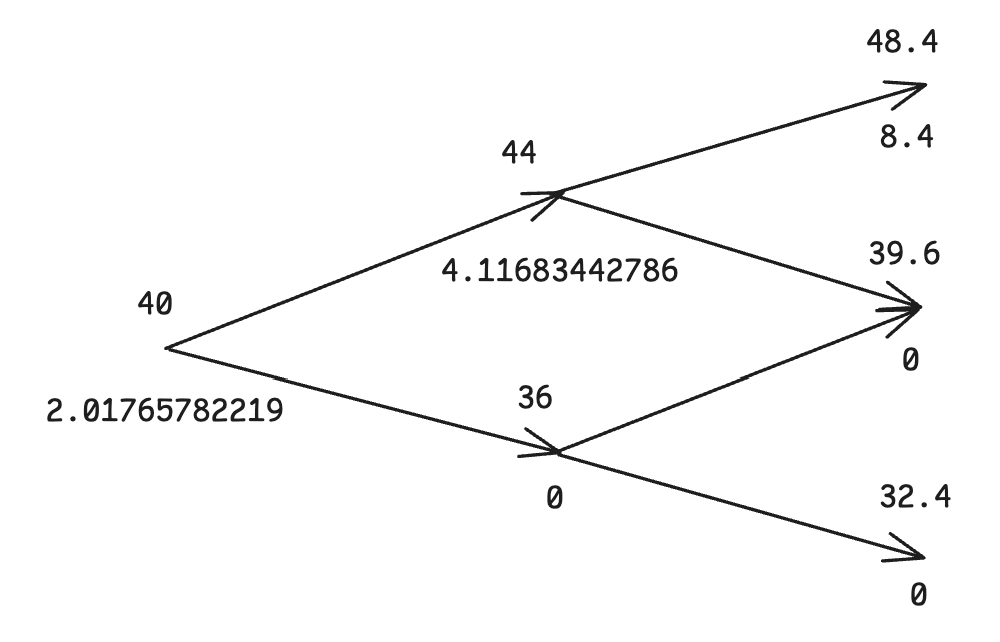
\includegraphics[width=400pt]{18_call_tree.png}
\end{figure}

\subsection*{(b)}
Checking at each node for early exrcise, the only ones of interest are the middle ones -- the lower middle one is at value 36 which is still below the strike price of 40, so there's no difference between the 0 payouts here. For the upper middle node, the expected payoff is 4.11683442786 while the early exercise payoff would be 44 - 40 = 4, so the early exercise is still not worth it. We therefore see that if the call were American, \boxed{\textbf{it would never be worth exercising early}}.

\subsection*{(c)}
We construct a similar tree as to part (a), except for puts, and solve accordingly. Starting with the top middle node:
\[
  e^{-0.08 \cdot \frac{3}{12}} \cdot (0.5 \cdot 0 + 0.5 \cdot 0.4) = e^{-0.02} \cdot 0.2 = 0.19603973466
\]
For the bottom middle node:
\[
  e^{-0.08 \cdot \frac{3}{12}} \cdot (0.5 \cdot 0.4 + 0.5 \cdot 7.6) = e^{-0.02} \cdot (0.2 + 3.8) = 3.9207946932
\]
And finally for the starting node and overall European put price: 
\[
  e^{-0.08 \cdot \frac{3}{12}} \cdot (0.5 \cdot 0.19603973466 + 0.5 \cdot 3.9207946932)
\]
\[
  = e^{-0.02} \cdot (0.09801986733 + 1.9603973466) = 2.01765782219 \approx \boxed{\mathbf{\$2.02}}
\]
\begin{figure}[h!]
  \centering
  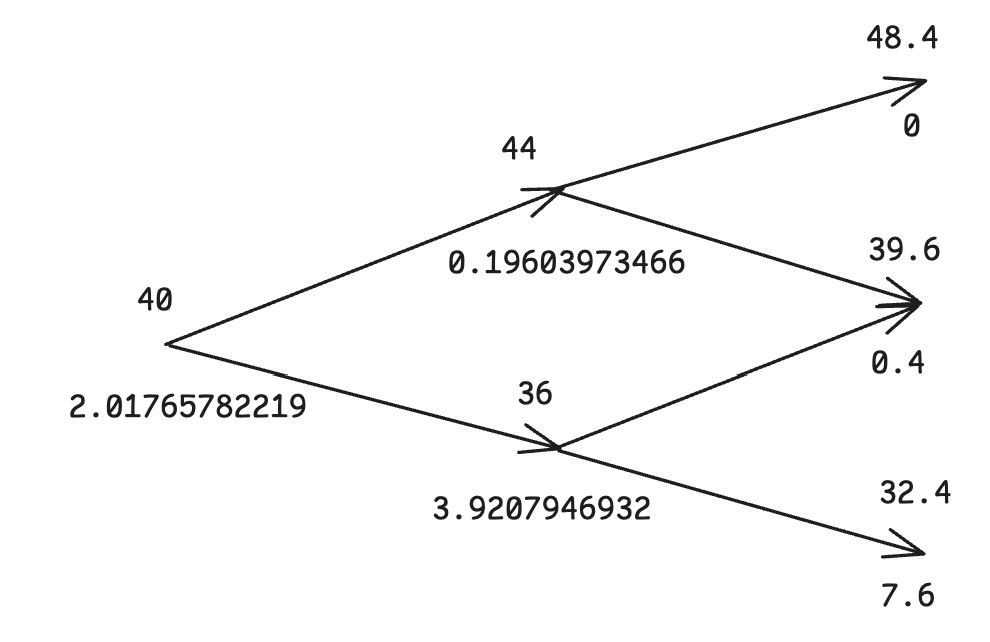
\includegraphics[width=400pt]{18_put_tree.png}
\end{figure}

\subsection*{(d)}
We start checking at each node for early exercises. At the upper middle node, it would not be as the price would be above the strike price, and there is a nonzero expected payoff there. For the lower middle node, however, we would have payoff if we exercised early of 40 - 36 = 4, which is greater than the expected payoff of 3.9207946932. So here it is indeed worth it to exercise immediately after the price goes down by 10\% the first time. We adjust the starting node payoff and price accordingly:
\[
  e^{-0.08 \cdot \frac{3}{12}} \cdot (0.5 \cdot 0.19603973466 + 0.5 \cdot 4) = e^{-0.02} \cdot (0.09801986733 + 2) = 2.05647629051 \approx \boxed{\mathbf{\$2.06}}
\]
which is higher value than the European option, which confirms that \boxed{\textbf{there does exist}} \boxed{\textbf{ a circumstance for which early exercise of the option is worth it.}}

}

\end{document}